

%\usepackage{graphicx}
\usepackage{hyperref}
\usepackage{todonotes}

\usepackage{endfloat}
\renewcommand{\efloatseparator}{\mbox{}} % no new page between figures

\usepackage{booktabs} % For formal tables

\settopmatter{printacmref=false} % Removes citation information below abstract
\renewcommand\footnotetextcopyrightpermission[1]{} % removes footnote with conference information in first column
\pagestyle{plain} % removes running headers

\newcommand{\TODO}[1]{\todo[inline]{#1}}



\title{Big Data Analytics in E-commerce}


\author{Himani Bhatt, Mrunal L Chaudhary}
\affiliation{%
  \institution{Indiana University}
  \city{Bloomington} 
  \state{Indiana} 
}
\email{himbhatt@iu.edu, mchaudh@iu.edu}



% The default list of authors is too long for headers}
\renewcommand{\shortauthors}{H. Bhatt, Mrunal C.}

\begin{abstract}
Humongous amounts of data gets generated every day in the domain of E-commerce industry. With the increasing competition and ever-changing market trends, it is a challenging task for the store owners to strategize business and marketing activities. If the companies are able to predict customer behavior, they can come up with business designs which can help them in making predictions about the customer purchasing patterns and thereby increase their revenue. In this project we have aimed to do analysis on the data of an E-commerce non-store online retail giant based in UK. The dataset, available in the UC Irvine repository by the name of `Online Retail', consists of the the goods purchased by different customers at a given time. Through this data available to us, we have done customer segmentation on the basis of the type and amount of goods purchased by a customer. We achieved this by doing a thorough exploration of the data, data pre-processing and then running different Machine Learning Classifiers to classify the customers in different categories.

\end{abstract}


\keywords{ HID $202$, HID $205$, i$523$, Machine Learning, Analysis, E-commerce, retail, Customer Segmentation, Python, Regression, Boosting, KNN, Random Forest.}

\maketitle

\section{Introduction}
The E-commerce industry is in constant shifts due to the ever-increasing changes in the technologies used to develop and maintain the E-commerce systems, the services that they are willing to offer, the market strategies which gain popularity at the time, and most importantly-  the customer behavior \cite{link1}. The online store owners are the ones who are most affected by these changes. And since the competition in the field of E-commerce is fierce, the online store owners need to come up with business strategies and technologies which provide better customer services leading to their satisfaction and earning customer loyalty. To achieve this, they need to address these ever changing issues to survive and thrive in the E-commerce market and come up with better decisions faster. The key to achieving this lies in better understanding of the customer behavior and their purchasing patterns. That is where analytics comes into play. Analysis of customer behavior and purchasing patterns helps in devising better and accurate marketing strategies which can not only help in generating more profits but also in saving both time and efforts that goes into trying and testing different marketing activities \cite{link1}. This ability to capture and analyze user data, and then provide useful and in depth insights in it is what Machine Learning empowers us with. In this project, we aim to do analysis on a data set `Online Retail' from the UC Irvine Machine Learning Repository to determine the customer purchasing pattern by using different machine Learning algorithms like K-Means Clustering, Logistic Regression, Random Forest, Gradient Boosting, etc.

\section{Background}
Before the advent of the World Wide Web, transactions that happened on a day to day basis meant physical presence of customers, the brick-and-mortar setting of a store which offered a limited variety of goods. With the evolution of internet and its application in retail, the field of E-commerce emerged and changed the entire facet of shopping. Since a proper set-up of a store is no longer needed, customers can buy goods at much lower prices, with a wider variety to choose from and that too without the need of physical presence. The online market is expected to grow by almost 56\% from the year 2015 to 2020 \cite{link2}. In the United States alone, 56\% of the population prefers to shop online. The E-commerce industry is growing at an average rate of 23\% every year, with 90\% of the Americans having done online shopping at some point in their lives \cite{link3}. With so many transactions happening over the internet, naturally the amount of data getting generated is humongous. Also, with the constantly changing market trends, strategies to overcome the competition and make profits need to be constantly improved. The key issues therefore are managing the data and drawing insights from them which will help in bettering the business decisions. To store and maintain the magnanimous amounts of data getting generated \emph{everyday} is a huge hassle, because along with the volume, this data gets generated at a break neck speed and in different formats from traditional numeric databases to unstructured text documents   \cite{link4}. The big data technologies like Hadoop and Spark can be used in addressing these hurdles, namely the volume, velocity and variety.

\subsection{The Three V's of E-commerce Big Data}
Like other technologies which deal with a humongous amount of data, E-commerce must also respond to the 3 Vs, namely Volume, Velocity and Variety:
\begin{itemize}
    \item Volume \\
    Thousand of online transactions happen every day making the data generation a real time process. The integration of Big Data involves collection of relevant data like customer behavior statistics on the basis of their searches, transactions, demography, etc. The challenge here is not only gathering the data but also in analyzing it.
    \item Variety \\
    The data from online transactions comes in different varieties, right from structured databases to unstructured text documents, videos, feedback emails and comments, and others. The retailers need to understand this for making the right business decisions by keeping a leeway for possible data fluctuations such as seasonal ad peak loads like Black Friday sales.
    \item Velocity \\
    Handling the huge amounts of data which is generated at unprecedented rates is another challenge that needs to be taken care of. It is therefore imperative to do rapid analysis so that timely actions can be taken to sustain in the competition and boost the profit margins \cite{link4}
\end{itemize}

Storing and maintaining the big data is a hassle in itself, but it will provide little value if proper analysis is not done on it. That is where we will be focusing on in this project - making sense of the data. Hence for the scope of this project, we have performed analysis on a small data set of around 45 MB. Machine Learning Algorithms learn from the data. Since we will be using Machine Learning Algorithms, the accuracy of Analysis will only increase with increase in the size of the dataset. We will be discussing this in further detail in the coming sections.\\
We have now established the fact that the E-commerce companies have a lot of data at their fingertips. Making use of this data is where the challenge lies. Machine learning is an approach by which insights can be drawn from digital data at a rate much faster than any human is capable of doing \cite{link5} . Following are some of the biggest challenges that are faced in the field of E-commerce which Machine Learning addresses successfully:\\
(1) \underline{Optimization of the Prices}:\\
Pricing, and in that, online pricing is critically important. Since prices of the competitors are only a few clicks away, it is far easier for the customers to compare prices. Setting up the optimum price, by considering many factors like the prices set by the competitors, the time of the day, the type of the customer and the product's demand therefore is a difficult task. Machine Learning technology can set the prices by considering all these factors at once.\\
(2) \underline{Fraud detection}: \\
The E-commerce industry, like the other industries, is susceptible to fraudulent activities. The consequences of these activities can lead to tarnishing the name of the company forever. Machine Learning helps in detecting and preventing the frauds by processing the repetitive data at a high speed.\\
(3) \underline{Search Ranking}: \\
Machine Learning is capable of pulling information from patterns of search and purchase by considering the factors like preferences, content and search items and come up with a powerful search engine that shows what the customer exactly wants. \\
(4) \underline{Product Recommendations}: \\
Machine Learning is capable of effortlessly quantifying the buying patterns of the customers and developing a recommendation engine which makes relevant product suggestions to them. \\
(5) \underline{Customer Segmentation and Personalization}: \\
In any business, Customer base is the most important factor and therefore providing a satisfactory customer experience is of utmost importance. The biggest challenge that E-commerce systems endeavor to overcome is the separation from their customers. In person, a salesperson can quickly take in what the customers are saying, their economic status, their body language, and behavior to help them find better or desired products. The salesperson thus is able to \emph{segment} customers, and provide them with a \emph{personalized} shopping experience. With online shopping, it is very difficult to make this happen since an in depth understanding is needed of the vast amount of the data to provide tailored choices to the customers, which can result in sale loss. \\
Machine Learning makes the biggest impact by making it possible to give personalized customer experiences which can boost the sales and thereby increase the revenue.\\ 
The type of analysis and Machine Learning Algorithm to be chosen depends solely on the data at hand. The data set we aim to analyze is a transnational data set that has been archived in the UC Irvine Machine Learning Repository under the name `Online Retail'. \\

A thorough Exploratory Data Analysis on this data lets us know what kind of Machine Learning Algorithm needs to be used. Also, several models can be applied and the one which gives the best accuracy and precision against the test data can be chosen. To add icing to the cake, we can even combine the results given by the different models to make an ensemble model which gives an accuracy that is better than that of the individual algorithms. Machine Learning Algorithms are mostly classified as supervised and unsupervised Learning algorithms.  \\
In Supervised Learning, each example is a pair of an input object and the corresponding output value, also called the supervisory signal. A supervised learning algorithm analyzed the training data to produce an inferred function which is used to map new, unknown output-value examples \cite{link6}. Since there is the output value to \emph{supervise} the learning algorithm, such approach is called `Supervised Learning'. The most commonly used Supervised Learning Algorithms are Logistic and Linear Regression, Bagging and Boosting Algorithms, Decision Trees and Random Forest. The Logistic Regression algorithm determines the relationship between the input and the output variables and generates a classifier model to predict the category to which a new example belongs to. Thus Logistic Regression is a classification algorithm \cite{link7}. Decision Trees are non parametric Supervised Learning Algorithms which create a model by learning simple decision rules inferred from data attributes to predict the value of a target variable. Decision Trees can be used either for Classification or Regression \cite{link8}. Bagging is a technique used to reduce the variance in the predictions by combining the result of multiple classifiers modeled on different sub-samples of the same data set. One of the most commonly and widely used implementation of Bagging is Random Forests. In Random forest, there are multiple trees which classify a new sample based on the set of attributes and a new sample is classified to that class which received the maximum `votes' from the individual trees. In case of doing Regression with the help of Random Forest, the average of the outputs given by different trees is taken  \cite{link9}.\\
In Unsupervised learning, only the input data is known with no knowledge of the corresponding output variable. The goal therefore of the Unsupervised Learning Algorithms is to model the underlying distribution or structure in the data to understand the data more. Since there is no output available to validate or `supervise' the answers, such learning algorithms are called Unsupervised. The most common application of unsupervised learning is clustering. Clustering enables to differentiate the data by discovering the inherent groupings of the input. The most common implementation of Clustering is the K-means algorithm. This algorithm works iteratively to assign each data point to one of the k-groups based on the feature similarity.

\section{Exploring the Dataset}

The dataset taken for the analysis is the `Online Retail' data set available on the UCI Machine Learning Repository. This is a transnational dataset which contains all the transactions occurring between 01/12/2010 and 09/12/2011 for a UK-based and registered non store online retail.The company mainly sells unique all-occasion gifts. Many customers of the company are wholesalers.\\

Data set consists of 5,41,909 transactions and 8 features which describe each of these transactions. There are missing values present in the dataset. All the attributes are integer and real numbers. The size of the dataset is 43.4 MB.\\

\subsection{Attribute Information}

\textbf{InvoiceNo}    : This refers to the Invoice number. It is a Nominal, 6-digit integral number uniquely assigned to each transaction. If this code starts with letter 'c', it indicates a cancellation. \\
\textbf{StockCode}    : This refers to the Product (item) code. It is a Nominal, 5-digit integral number uniquely assigned to each distinct product.\\
\textbf{Description}  : This refers to the Product (item) name. It is of Nominal data type. \\
\textbf{Quantity}     : This refers to the The quantities of each product (item) per transaction. It is Numeric in type.\\
\textbf{InvoiceDate}  : This refers to the Invoice Date and time. It is Numeric,and represents the day and time when each transaction was generated. \\
\textbf{UnitPrice}    : This refers to the Unit price. It is of Numeric type, and represent the Product price per unit in sterling. \\
\textbf{customerID}   : This refers to the Customer number. It i a Nominal, 5-digit integral number uniquely assigned to each customer.\\
\textbf{Country}      : This refers to the Country name. It is of Nominal type, and represents the name of the country where each customer resides.\\

\section{Data Preparation}

\subsection{Installation Steps}
The project has been implemented in Python 2.7 version and we have used the Jupyter Notebook App for the program execution. The Jupyter Notebook Application is an application having server-client architecture which allows editing and executing notebook documents through a web browser. A notebook document is a human readable and machine executable document which can be executed for implementation of data analysis. The Jupyter Notebook Application can be executed on the local host or can be installed on a remote machine accessed via the internet \cite{link15}. \\
The Jupyter Notebook can be installed very easily on a machine which has either Python $2$ or Python $3$ version. Since we have implemented our project in Python 2.7, following commands are to be run in the terminal:\\
pip install --upgrade pip \\
The above command will upgrade the Python package manager (pip).
pip install jupyter \\
The above command will install Jupyter in the local machine.\\
Once the Jupyter Notebook has been installed, it can be run using the following command in the terminal:\\
jupyter notebook\\
This command will run the Jupyter notebook in the default browser of the machine on the default port $8888$ of the localhost.

\subsection{Packages Installation}
Before running the code the following packages were imported/installed in the Python environment.

\begin{itemize}
    \item pandas
    Pandas provide a very fast and flexible data structures to make working with relational data easy and fairly intuitive.
    \item numpy
    This is a fundamental package for scientific computation with Python and can be used as an efficient multi-dimensional container of generic data.
    \item sklearn
    Scikit-learn makes a wide range of supervised and unsupervised machine learning algorithms  available in python. We have implemented all the Machine Learning Algorithms using this library.
\end{itemize}


\subsection{Null Value Treatment}
Before going ahead with Data Exploration, a quick look through the data showed many missing values. Hence before doing any analysis, it is imperative to treat the missing values. The dataset has almost 25\% of the entries that are not assigned to any of the customer i.e. customerID attribute for those entries is null. \\
Missing value treatment can be done by deleting the columns and/or rows which have missing values beyond a decided threshold, or replacing them with the attribute mean, median or mode. 
Since the missing values in our case is the customerID, the replacement method cannot be applied. Also, these entries are useless for the analysis since we aim to do Customer Segmentation and without knowing the customerID, it cannot be achieved. Hence we have deleted the rows with missing customerID. After removing these entries , the dataset left is with 4,06,829 transactions.\\

The content of the dataset appears as shown in the figure \ref{data}.

\begin{figure}[H]
\caption{Data set Contents}
\label{data}
\centering
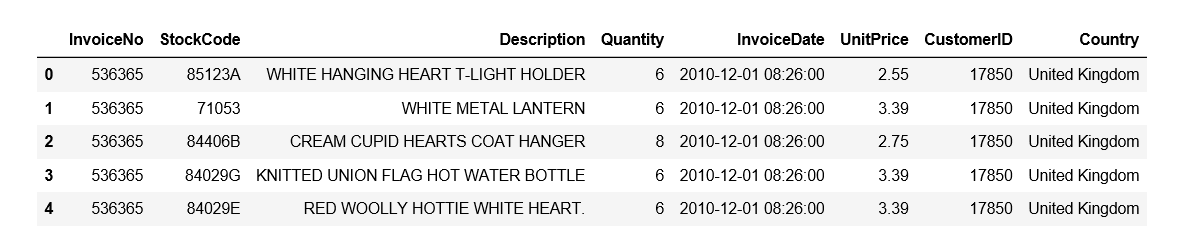
\includegraphics[width=0.5\textwidth]{images/DatasetContent.PNG}
\end{figure}

We also removed the duplicate values present in the dataset. There are 5225 such entries present in the data set that are deleted.\\

\section{Exploring the content of variables}

The dataframe has 8 variables and we can draw some inferences by analyzing these variables.

\subsection{Countries}

From the data we can see that there are 37 different countries from which orders were placed. We can determine the number of orders per country by a  `Chloropeth' map. A Chloropleth map uses different colors and shades within predefined areas to indicate quantities in those areas. \\

\begin{figure}[H]
\caption{Distribution of Orders based on Countries}
\label{country}
\centering
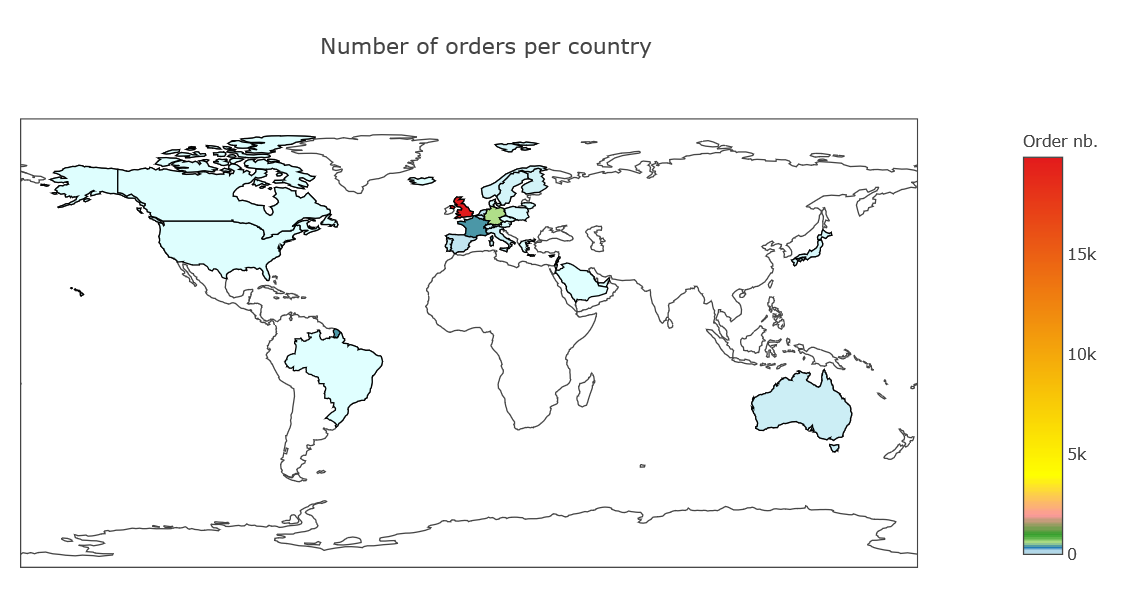
\includegraphics[width=0.5\textwidth]{images/chloropleth.PNG}
\end{figure}

The figure \ref{country} shows that maximum number of orders are placed from UK.

\subsection{Customers and products}

On observing the number of users, products purchased and number of transactions made; we can see that these are not proportional. This suggests that there were many transactions made for cancelling the orders.\\

\begin{figure}[H]
\caption{Customer Products Transactions}
\label{2.1}
\centering
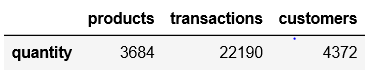
\includegraphics[width=0.5\textwidth]{images/2_1.PNG}
\end{figure}

We can also determine the number of products purchased in each transaction. It shows that some customers purchased goods in bulk whereas some purchased a single product in a transaction.
Also the orders with InvoiceNo starting with C are the cancelled orders.

\begin{figure}[H]
\caption{Number of products per Customer}
\label{2.2}
\centering
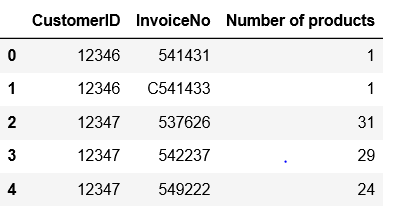
\includegraphics[width=0.5\textwidth]{images/2_2.PNG}
\end{figure}

\subsection{Cancelled Orders}

Almost 16\% (3654) of the transactions are corresponding to the cancelled orders. In the dataset, corresponding to each cancelled transaction we should have an order placed with same quantity of products requested. While checking the same in the dataset, we found the following for some of the orders.\\

\begin{figure}[H]
\caption{Transactions for Cancellation}
\label{2.3}
\centering
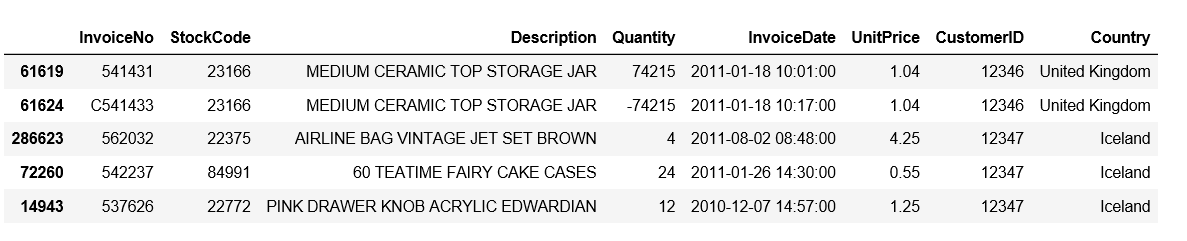
\includegraphics[width=0.5\textwidth]{images/2_3.PNG}
\end{figure}

This hypothesis should apply to the complete dataset, but on checking the whole dataset it is found out that there are some cancelled orders without the purchase order (the history of the order) made. This is done by locating the entries that indicate a negative quantity and then checking if there is an order indicating the same quantity (but positive) with the same description and the same customerID. We still get negative quantities. Going deeper in to this suggests that the entries with description `Discount' have negative quantities associated with that transaction. And hence, to do the verification, we eliminated the 'Discount' entries. But again the initial hypothesis do not match; we still have negative numbers appearing in the quantity.\\
This can be because the buy orders were performed before December 2010 (the point of entry of the database). We can delete the records where a cancel order exists without the corresponding purchase order or where there is at least one counterpart with the exact quantity (since both records are logically cancelling each other).Total 8795 such records are found and deleted from the dataset.\\

\subsection{StockCode}

The StockCode variable should ideally contain letters. So we have filtered out the codes with only letters. We can observe the different type of transactions based on these (example D is for discounted transaction).\\

\begin{figure}[H]
\caption{Stock Codes}
\label{2.4}
\centering
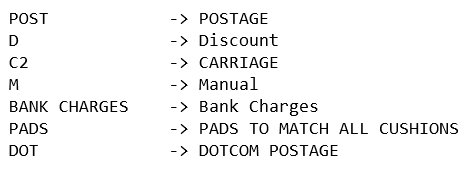
\includegraphics[width=0.5\textwidth]{images/2_4.PNG}
\end{figure}

\subsection{Basket Price}

We have added a new variable to indicate total price of the purchase (by multiplying unit price of each product with quantity purchased). Each transaction corresponds to the prices for a single product. On grouping the records based on a single order, we can see the complete price for that order.\\

\begin{figure}[H]
\caption{Basket Price}
\label{2.5}
\centering
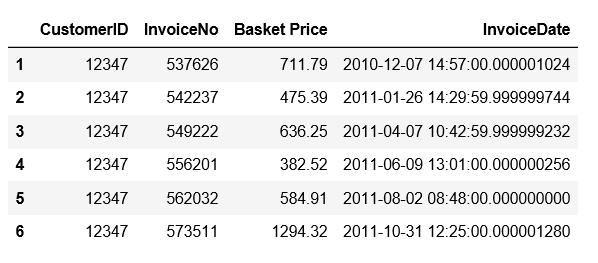
\includegraphics[width=0.5\textwidth]{images/2_5.PNG}
\end{figure}

We can visualize the orders distinguished on the basis of total price of the basket. It can be shown using a pie-chart.

\begin{figure}[H]
\caption{Pie-Chart}
\label{2.6}
\centering
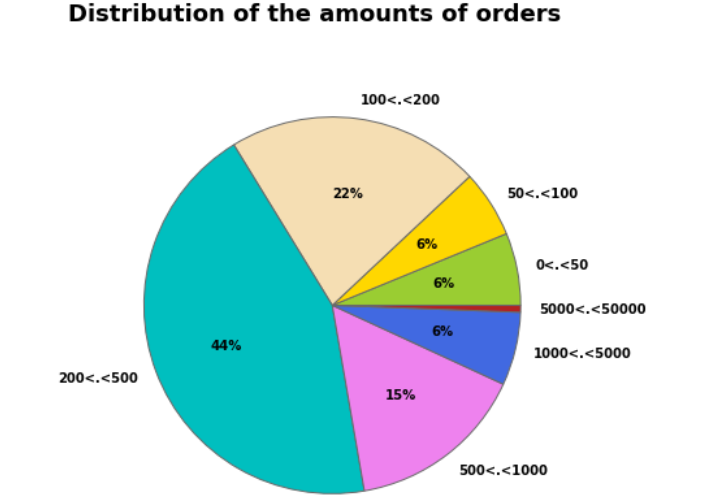
\includegraphics[width=0.5\textwidth]{images/2_6.PNG}
\end{figure}

It shows that majority of the orders are the bulk purchases since 60\% of the orders have amounts greater than 200 Sterling.

\section{Exploring Product Categories}

The dataset contains two variables- Stockcode and Description defining products. We can categorize the products based on the content of the description variable. This can be done in the following way :\\

\begin{itemize}
  \item Extracting the proper or the common names appearing in the products description.
  \item Extracting the root of the word and combining sa et of names associated with this particular root.
  \item Finding the frequency of root in the dataframe.
 \end{itemize}
 
 We found that there are 1483 keywords present in the description variable of the dataset. The most common keywords can be determined based on the occurrences. The figure \ref{3.1} shows the top word occurrences.
 
 \begin{figure}[H]
\caption{Word Occurrences}
\label{3.1}
\centering
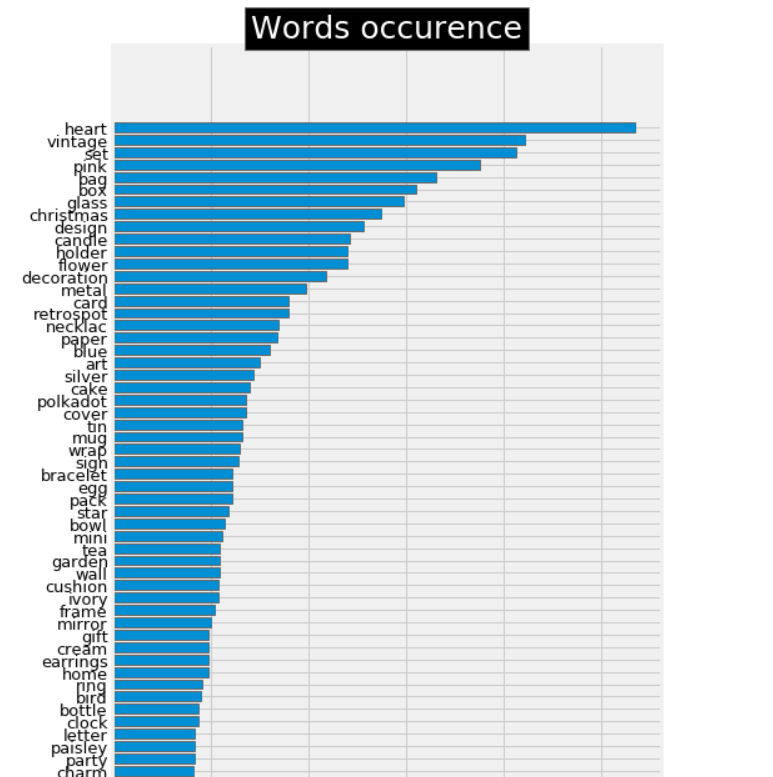
\includegraphics[width=0.5\textwidth]{images/3_1.PNG}
\end{figure}

\subsection{Categorizing Products}

We have obtained around 1400 keywords from the above occurrence list , most of which do not make sense. After discarding the keywords that are appearing less than 13 times, we are left with 193 keywords that we will consider for our analysis.\\

These significant keywords are used for creating categories of the products. The data has been encoded using the principle of one-hot-encoding.\\

\textbf{One hot encoding} - One hot encoding is a process by which categorical variables are converted into a binary format of 0's and 1's that could be provided to ML algorithms to do a better job in prediction. The words present in the descriptions of the products are encoded. Also price range column is added as it will help in balanced grouping of the products.\\

\subsection{Clustering of products}

In the previous step we have created a matrix with encoded version of words present in the description variable. K-means clustering is used for the cluster assignment and since the data is in binary format because of encoding, the most appropriate distance method will be Hamming's metric (other distance functions are euclidean distance, Manhattan distance, binary distance, etc). It basically measures the minimum number of substitutions required to change one string into the other. But since the k-means package available in sklearn uses Euclidean distance by default, we have used it for our analysis.\\

\underline{Selection of optimum K-value}\\

The number of clusters can be selected using silhouette analysis on K-means clustering. It is used to study the separation distance between the resulting clusters. The silhouette plot displays a measure of how close each point in one cluster is to the points in the neighboring clusters and thus provides a way to assess parameters like number of clusters visually. This measure has a range of [-1, 1].\\
Silhouette coefficients (as these values are referred to) near +1 indicate that the sample is far away from the neighboring clusters. A value of 0 indicates that the sample is on or very close to the decision boundary between two neighboring clusters and negative values indicate that those samples might have been assigned to the wrong cluster.\\

The figure \ref{3.2} shows silhouette score for different values of k. These scores do not have significant differences, but since for k value greater than 5, the resulting clusters have very few elements in them, we have taken k as 5. 

\begin{figure}[H]
\caption{Silhouette Scores}
\label{3.2}
\centering
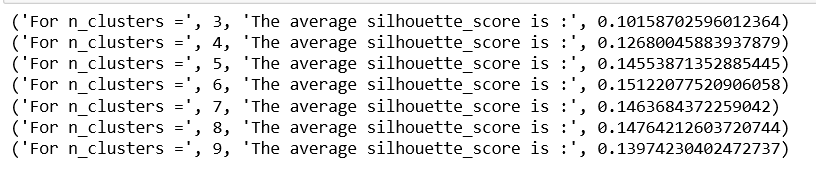
\includegraphics[width=0.5\textwidth]{images/3_2.PNG}
\end{figure}

\subsection{Validating Quality of Classification}

\subsubsection{\textbf{Silhouette Score}}

From the silhouette plot we can see that cluster 1 has more number of elements than the other clusters. But overall distribution of elements in the clusters is comparative. Same can be seen from the figure \ref{3.4}.

\begin{figure}[H]
\caption{Silhouette plot}
\label{3.3}
\centering
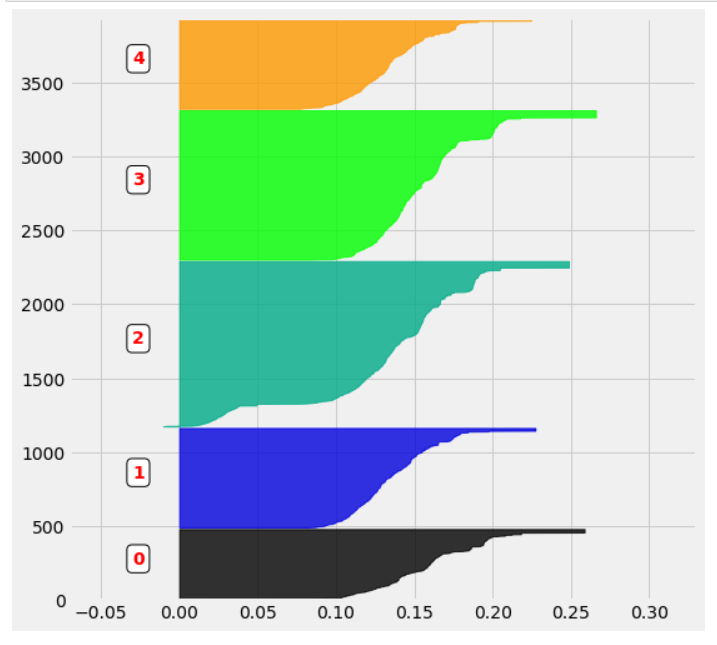
\includegraphics[width=0.5\textwidth]{images/3_3.PNG}
\end{figure}

\begin{figure}[H]
\caption{Cluster Composition}
\label{3.4}
\centering
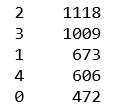
\includegraphics[width=0.5\textwidth]{images/3_4.PNG}
\end{figure}

\subsubsection{\textbf{Principal Component Analysis}}

The main idea of principal component analysis (PCA) is to reduce the dimensionality of a data set consisting of many variables correlated with each other, either heavily or lightly, while retaining the variation present in the dataset, up to the maximum extent. The initial matrix has large number of variables and hence, PCA is used for dimensionality reduction. From the figure we can say that we need more than 100 components to explain 90\% of the variance in the data.\\

\begin{figure}[H]
\caption{PCA}
\label{3.5}
\centering
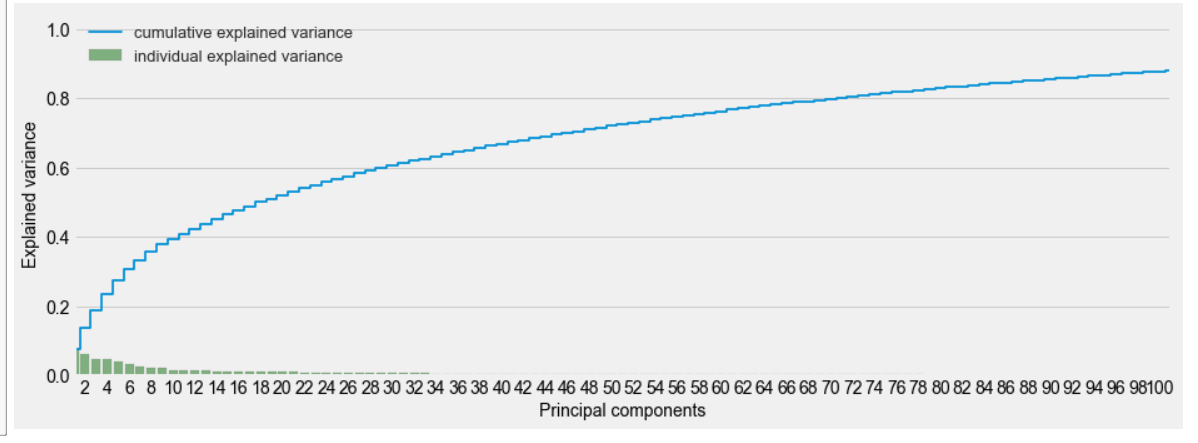
\includegraphics[width=0.5\textwidth]{images/3_5.PNG}
\end{figure}

Another application of PCA is that it sets the indication of “cluster” membership. Biplot is the best example that can be provided here to support this idea. Using biplot, we get the indication of number of clusters in a dataset. Below figure \ref{3.6} shows these on limited number of components (since it is only for visualizing cluster distribution). We can observe the groupings of points or clusters as expected.\\

\begin{figure}[H]
\caption{Biplot}
\label{3.6}
\centering
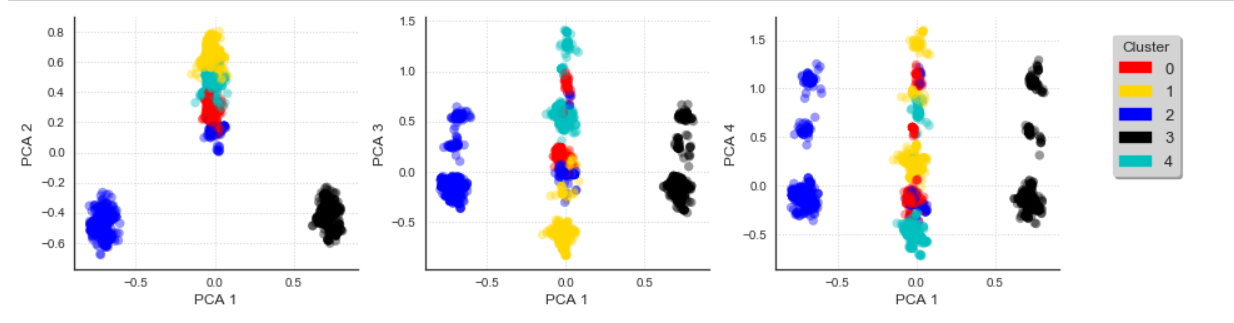
\includegraphics[width=0.5\textwidth]{images/3_6.PNG}
\end{figure}

\section{Exploring Customer Categories}


In the previous section, we have divided products in 5 clusters. We have added a dummy variable categ\_product to indicate the cluster to which that customer belongs. Based on the clustering done on products we have created variables categ\_0..4 which stores amount spent on each of the product category. And the categ\_product variable which we have just created will have initial cluster assignment based on these variables. These can be further grouped on the basis of InvoiceNo.\\

\begin{figure}[H]
\caption{Table}
\label{4.1}
\centering
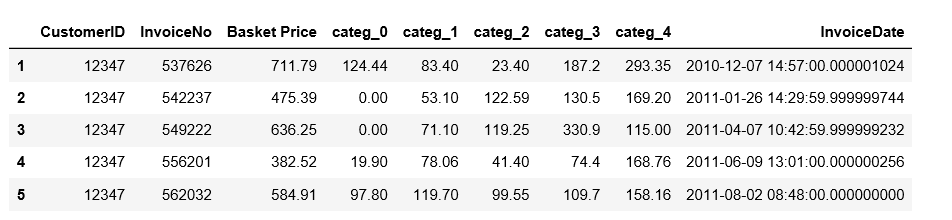
\includegraphics[width=0.5\textwidth]{images/4_1.PNG}
\end{figure}


\subsection{Subsetting dataframe based on Time}


We have taken 12 months data for the analysis. This can be done on the basis of variable InvoiceDate present in the dataset. Using this data we have developed a model to characterize and anticipate the habits of customers using the site and this, we are doing it from the first visit.\\

In the previous section we have seen the basket price of each invoices. For further analysis we will combine these on the basis of customerID to analyze the number of purchases made by each customer. A customer category of particular interest is that of customers who make only one purchase. So one objective may be, for example, to target these customers in order to retain them. In the dataset we have almost one-third of the customer base similar to this.

\begin{figure}[H]
\caption{Number of Purchases}
\label{4.2}
\centering
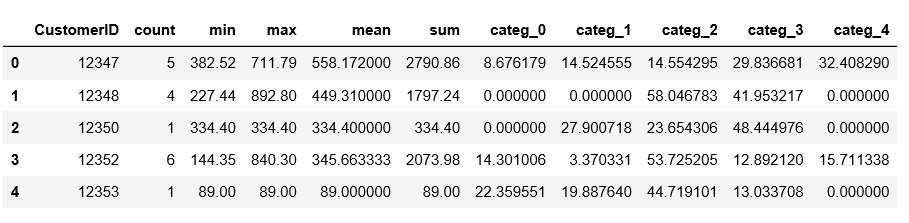
\includegraphics[width=0.5\textwidth]{images/4_2.PNG}
\end{figure}


\subsection{Categorizing Customers}

The information transactions per user is used for characterizing different types of customers. Because of different ranges of variations of different variables we have first scaled the data set. As done in the case of product categorization, we have again used K-means algorithm for cluster assignment.\\

Using the silhouette score, the optimum value of k comes out to be 11. The assignment of customers into different clusters is shown in figure \ref{4.3}

\begin{figure}[H]
\caption{Number of Purchase}
\label{4.3}
\centering
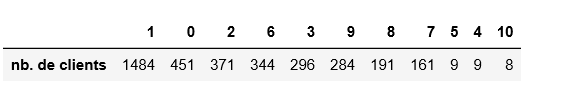
\includegraphics[width=0.5\textwidth]{images/4_3.PNG}
\end{figure}

Now we will check validity of the cluster assignment using PCA and Silhouette plot as done in the case of product categorization.\\

\subsubsection{\textbf{PCA}}

There is a certain disparity in the sizes of different groups that have been created. So we have validated it using PCA. From the representation, it can be seen, for example, that the first principal component allow to separate the tiniest clusters from the rest. More generally, we see that there is always a representation in which two clusters will appear to be distinct.\\


\begin{figure}[H]
\caption{PCA}
\label{4.4}
\centering
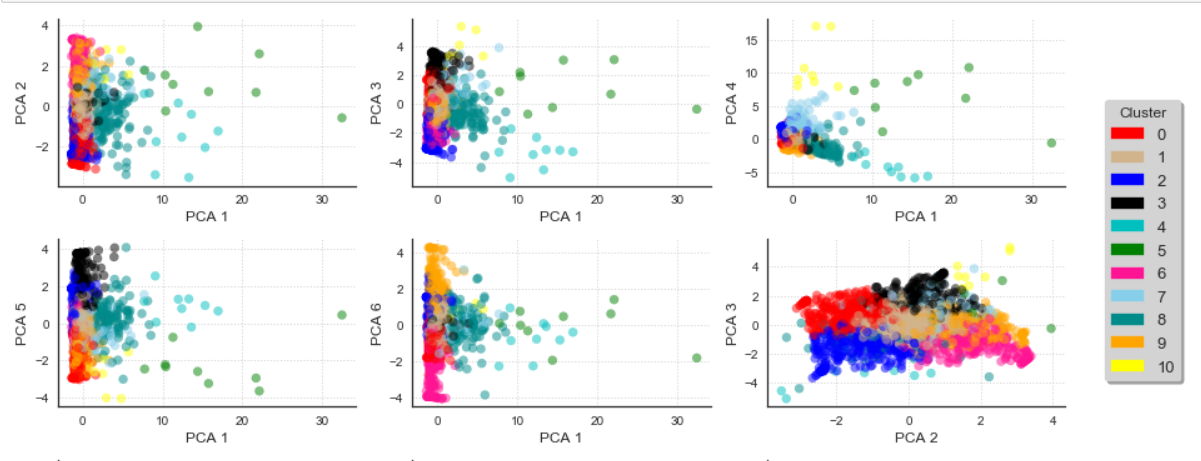
\includegraphics[width=0.5\textwidth]{images/4_4.PNG}
\end{figure}

\subsubsection{\textbf{Silhouette Plot}}

As with product categories, another way to look at the quality of the separation is to look at silhouette scores within different clusters:\\

\begin{figure}[H]
\caption{Silhouette Plot}
\label{4.5}
\centering
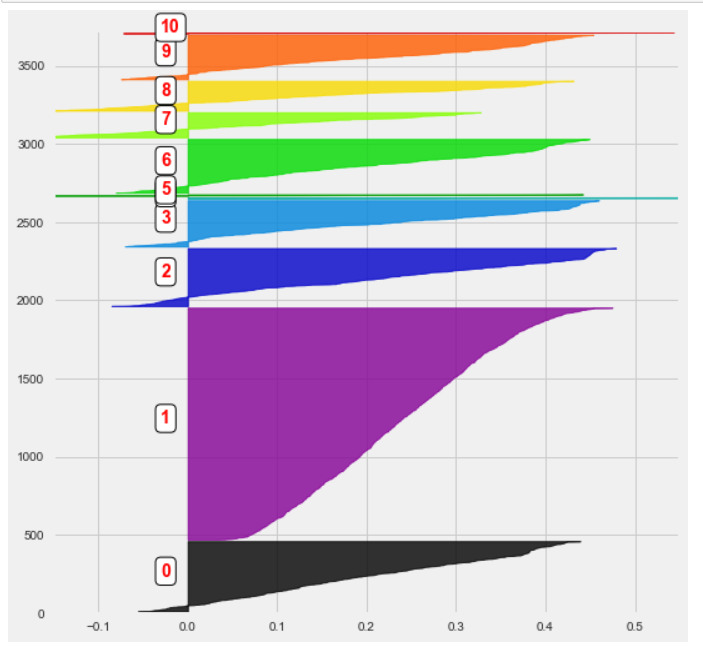
\includegraphics[width=0.5\textwidth]{images/4_5.PNG}
\end{figure}

We can see that the different clusters are indeed disjoint.

\section{Classification of Customers using Classification Algorithms}

In the previous section, we have made different client categories. In this part we will adjust a classifier so that the consumers can be classified in different client categories. The main aim of this is to enable the Classification on the first visit of the customer. To do this, we have defined a class that will allow interfacing the common functionalities to the different classifiers. Since we are going to classify the client on the basis of his/her first visit, the only parameters that we take into consideration are the contents of the basket and not the frequency of visits or the variation in the basket price over a period of time. Once this is done, we have split the dataset into train and test sets. The classification algorithms which we used to do this are mentioned below.\\
Before we delve deeper into the Classification Algorithm, some important concepts that need to be addressed are Cross Validation, Bias, Variance, underfitting and overfitting of the model.
\begin{itemize}
    \item Variance:
    Variance essentially means how much the models estimated from the different training sets differ from each other. It measures how much the predictions made for a given point vary between the different realizations of the model \cite{link17}. When the training data tries to fit all the sample points to define the model, even the outlier data points, which are nothing but the noise, affect the model. Usually, the variance increases with increase in the complexity of the model.
    \item Bias:
    Bias essentially means how much the average model over the training sets differ from the true model. Bias usually occurs if the model is over simplified or if some inaccurate assumptions are made. Thus Bias increases with increase in the over simplification of the model \cite{link17}.
    \item Underfitting:
    Underfitting occurs when the model is too simple to make relevant classification of the testing data \cite{link17}.Thus when a model possesses high bias and low variance, we say there is underfitting of the model.
    \item Overfitting
    Overfitting of a model occurs when the model is too complex and tries to fit in the irrelevant/outlier datapoints from the training set which is nothing but the noise \cite{link17}. Thus when a model possesses low bias and high variance, we say there is overfitting of the model.
    \item Cross Validation: \\
    Cross Validation is a technique for evaluating the predictive models by partitioning the original dataset into a training set to train the model, and a testing set to evaluate the model \cite{link16}. There are different ways to implement Cross Validation, the most effective of them all is the K-fold Cross Validation. In this method the dataset is divided into k subsets, out of which one is used as the test data and the remaining $k-1$ are combined together to form training data. This process is done k times, ensuring that every single sample in the dataset gets to be tested exactly one time and gets trained upon exactly $k-1$ times. The variance therefore gets decreased as the k increases \cite{link16}.
\end{itemize}

Thus it can be said that a model will always be associated with variance and bias. If the bias is low then the variance is high, as in the case of the complex models. And if the bias is high then the variance is low as in the case of simplified models. Hence there is always a trade off between these two kinds of errors. This is called the Bias-Variance trade-off. We are interested in a model with low variance and low bias.


\subsection{Logistic Regression}
Logistic Regression as mentioned before is a Supervised Learning method which does analysis on a dataset containing two or more independent variables for determining the outcome. This outcome, i.e the dependent variable, is binary in nature, meaning it can have only two possible outcomes \cite{link10}. Multinomial Logistic Regression as the name suggests, generalizes the Logistic Regression to multiple classes, meaning the model can be used to predict the probabilities of the different outcomes of a categorically distributed dependent variable \cite{link111}. The goal of a Logistic Regression model is to determine a fitting model which best describes the relationship between the dependent variables (output variable) and a set of the input independent variables. Logistic Regression generates the coefficients along with the standard errors and significance levels of the below equation for predicting the logit transformation of the probability of presence of the characteristics of interest in a given sample example \cite{link10}. \\

$logit(p) = \beta_0 + \beta_1X_1 + \beta_2X_2 +\beta_3X_3 + \beta_4X_4 + .... + \beta_kX_k$

where p is the probability of the presence of a characteristic of interest.
and $logit(p) = log(p/1-p)$
In logistic Regression, the goal is to choose the parameters $\beta$ in such a way that the likelihood of observing the new sample values is maximized \cite{link10}.\\
In the Python code, we have imported the module `linear\_model' from the `sklearn' package to perform Logistic Regression by using the function `logistic\_regression'. And we have taken the $k=5$ for k-fold cross validation. While performing Logistic Regression, we created an instance of the Class\_Fit class and then ran the model on training data and see how the predictions are made as compared to the real values. The learning curve graph is as shown in Fig 20.

\begin{figure}[H]
\caption{Logistic Regression Learning Curve}
\label{5.1}
\centering
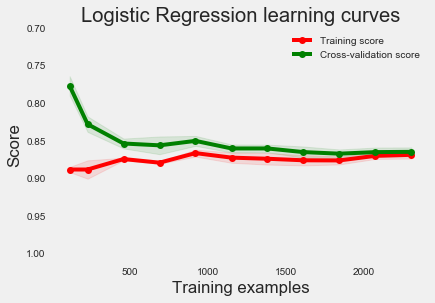
\includegraphics[width=0.5\textwidth]{images/5_1.png}
\end{figure}

As we can see from the figure \ref{5.1}, when the number of training examples increases, the cross-validation and train curves almost converge towards the same limit suggesting that the model has low variance. Thus we can say that model is not suffering from over-fitting. Also one point to note is that the accuracy is high, which means that the model has low bias, thus suggesting that it does not under-fit the data. The precision which we got from running the Logistic Regression model on the training data is 88.78\%.

\subsection{K Nearest Neighbours}
KNN is a non parametric algorithm which means that there are no underlying assumptions that are made on the data. Also it is a lazy learning algorithm meaning that it does not do any generalization by using the training data. All the training data is needed during the testing phase \cite{link11}.\\
KNN makes predictions using the training dataset directly. Predictions are made for a new instance (x) by searching through the entire training set for the K most similar instances (the neighbors) and summarizing the output variable for those K instances. For regression this might be the mean output variable, in classification this is be the model (or most common) class value. To elaborate on this, KNN makes predictions using the training dataset directly. These predictions are made for a new sample by going through the entire training set to find k such samples which are most similar or which are the `neighbors' of the the new instance. Once these k instances are found out, the output variable corresponding to these is summarized and in case of Classification, it gives a class value to which the new instance belongs. The k `neighbors', i.e., the most similar instances from the data set are found by using the distance measure- k such instances whose distance from the new instance is the least \cite{link11}. There are many distance functions which can be used, the most popular being the Eucledian distance function, the formula for which is given by:

$EuclideanDistance(x, x_i) = sqrt( sum( (x_j-x_ii)^2 ) )$

where x is a new data point and $x_i$ is an already existing point \cite{link11}.\\
The optimum value of K can be found by algorithm tuning, i.e. running the algorithm over several values of k and finding out and then figuring out for which k the algorithm gives the best results \cite{link12}.\\
The output, i.e the class of the new sample can be calculated as the class which has the highest frequency from the k neighbours. Thus, each of the instances votes for their own class and the class which gets the maximum votes is taken as the prediction value \cite{link12}. \\
In Python, the `neighbors' library is imported from the sklearn package which performs the KNN classification through the Kneighborsclassifiers function. The parameters that are used are 'n\_neighbors' which represents the number of neighbors to use, in our case we have used the np.arrange method to give  sequence from 1 to 49. Also, we run the model using the K-fold Cross Validation with the value of $k=5$. Once the model is run, we have drawn the learning curve graph which is as represented in the Fig 21. 

\begin{figure}[H]
\caption{KNN Learning Curve}
\label{5.2}
\centering
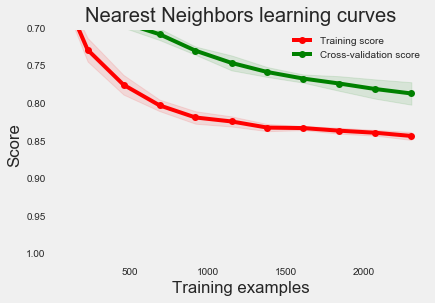
\includegraphics[width=0.5\textwidth]{images/5_2.png}
\end{figure}

The precision which we got from running the KNN model on the training data is 80.33\%.

\subsection{Random Forest} 
As the name suggests, Random Forest is an ensemble classifier which consists of many classification trees. An ensemble classifier is a multiple classifier algorithms, decision trees in the case of Random Forests, and the final output is the combined output of the all the classifier algorithms. In our case we will be using Random Forest Algorithm for classification of the clients into different categories. A Random Forest grows many trees. For classifying a new object from an input vector, each tree in the forest gives a classification and vote for a particular class. And the forest then chooses the class having maximum number of votes over the other classes \cite{link13}.\\
The question here that needs to be addressed is, how does the growth of a tree happen?\\
Each tree is grown as follows:\\
If the training set consists of N cases, then N cases are sampled with replacement from the original data. This is the training set for growing a tree. Thereafter, a number m<<M which is the number of input variables is taken such that the best split obtained on these m is used to split the node. The value of m is constant throughout the forest-growing. Each tree is allowed to grow to the fullest possible extension \cite{link13}.
In Python, the `ensemble' library is imported from the sklearn package which performs the Random Forest classification through the RandomForestlassifier function. The parameters given to this function are criterion, n\_estimators and max\_features. The criterion is used to measure the quality of the split. The Gini is for measuring the Gini impurity and Entropy is for information gain. The max\_features are the number of the features that can be chosen when looking for the best split. For `sqrt', the number of maximum features chosen are square root of the number of the features and for `log', it is log of the number of the features. And the n\_estimators is the number of trees in the forest.Once the model is run, we have drawn the learning curve graph which is as represented in the \ref{5.3} .

\begin{figure}[H]
\caption{Random Forest Learning Curve}
\label{5.3}
\centering
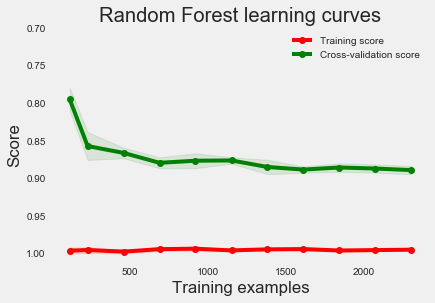
\includegraphics[width=0.5\textwidth]{images/5_3.png}
\end{figure}

The precision which we got from running the Random Forest model on the training data is 90.17\%.


\subsection{Gradient Boosting Classifier}
AdaBoost Classifier, short for Adaptive Classifier is another example of ensemble classifier. 
It is a general ensemble method which creates a strong classifier by combining the outputs of the weaker learning algorithms into a weighted sum to finally provide the output of the \emph{boosted} classifier. This is done by building one model from the training set and then building a second one which attempts to rectify the errors from the first model and so on until either the limit of maximum models that can be added is reached or the training set is predicted accurately. AdaBoost is an adaptive algorithm, meaning that the weak learning algorithm can be tweaked to create a stronger classifier \cite{link15}. \\
The Adaptive Boosting algorithm was recast into a statistical framework. ``Arcing is an acronym for Adaptive Re-weighting and Combining. Each step in an arcing algorithm consists of a weighted minimization followed by a re-computation of [the classifiers] and [weighted input] \cite{link15}''
This framework is called as Gradient Boosting. \\
Gradient Boosting involves three elements namely:
\begin{itemize}
 \item{A loss function to be optimized}
 The selection of the loss function depends on the problem at hand. For example if it is a regression algorithm, then squared loss functions are used and if it is a classification algorithm then logarithmic functions are used.
 \item{A weak learner for making predictions}
 Regression trees are used as the weak learners in the Gradient Boosting Algorithm since they can output real values for splits which can be added together and the residuals in the predictions can be corrected. These trees are constructed in a greedy manner usually up to 4-8 levels.
 \item{An additive model to add weak learners to minimize the loss functions}
 The trees are added one at a time with no changes to the existing trees in the model. A gradient descent model is used to reduce the loss when adding trees first by parameterizing the tree and then by modifying the parameters of the tree and moving in the right direction by reducing the loss in residuals. This approach is called Functional Gradient descent \cite{link15}.
\end{itemize}

This framework was further developed by Friedman and called Gradient Boosting Machines. Later called just gradient boosting or gradient tree boosting \cite{link15}.\\
In Python, the `ensemble' library is imported from the sklearn package which performs the Gradient Boosting classification through the GradientBoostingClassifier function. The parameter given to this function is n\_estimators which is the number of boosting stages to perform. Gradient boosting is fairly robust to over-fitting so a large number results in better performance.

\begin{figure}[H]
\caption{Gradient Boosting Learning Curve}
\label{5.4}
\centering
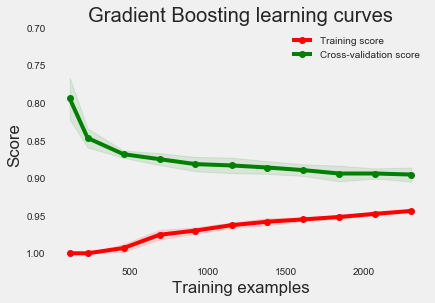
\includegraphics[width=0.5\textwidth]{images/5_4.png}
\end{figure}

The precision which we got from running the Gradient Boosting model on the training data is 90.86\%.

Now that we have the results of all the models, we can combine them using VotingClassifier method that we imported from the sklearn package to improve the classification model. Since we have already found the best parameters for each of the classifiers, we have adjusted the parameters of the classifiers accordingly. So now the best parameters are taken and merged to define a classifier which  we then trained on the data. When we created a prediction on this, we got the precision value as 90.44\%.

\section{Testing the predictions}
Until now we have done all the analysis on the data from the first 10 months. After this we test the model on the set\_test dataframe which contains the data of the last two months. The regrouping of the data is done according to the same procedure that we followed while regrouping the training data. But now we have to take into consideration the time difference in between the two datasets and the count(the total number of visits which the client made to the website) and sum(total amount that he/she spent) variables so that we have an equivalence in between the training set and testing set. The dataframe so obtained is now converted to a matrix and we retained only those variables that define the category to which the clients belonged. And just like on the training dataset the method of normalization was called, to maintain consistency, the same method is called on the test set as well.\\
Each row of the matrix obtained now represents the buying habits of the customers. Now all we have to do is to define the category to which the customer belongs by using these habits. The important point to note here is that this is just the test data preparation step by defining the category to which the consumer belongs for a period of two months through the variables count, min, max and sum. Thus this step \emph{does not} correspond to the classification step itself. The classifier that we defined in the step 5 uses variables that were defined from the client's first purchase.\\
So now, we have the data available for two months, and through that we can define the category to which the consumer belongs. The predictions now obtained by running the classifiers on test data can be tested against these categories. The instance of the k-means clustering method that we used in the Customer Categories section is used to define the category to which a client belongs. This contains the predict method which will calculate the distance of the consumers from the centroids of the 11 categories that we deduced, and the category which is closest to the clients' buying habits will define his/her category. Thus all we need after this for the execution of the classifier is to select the variables on which it acts, i.e. on mean, cat\_0, cat\_1, cat\_2, cat\_3 and cat\_4. After examining the predictions of the different classifiers, we get precision scores as follows:\\ 
\begin{center}
 \begin{tabular}{|c | c|} 
 \hline
 Algorithm & Precision(\%) \\ [0.5ex] 
 \hline
 Logistic Regression & 72.99\\ 
 \hline
 KNN & 68.44 \\
 \hline
 Random Forest & 75.93 \\
 \hline
 Gradient boosting & 75.74 \\
 \hline
 
\end{tabular}
\end{center}

And now, like we did in the Section 5, we will use the voting classifier method to merge the results obtained by these individual classifiers and see whether they combined result is better than the individual. It turns out that it is. We get the precision rate for the combined classifier to be 76.48\% for the test data set. This concludes the analysis phase.\\

\section{Conclusion}
E-commerce is one of the emerging fields for Data Analysis since a lot of data gets generated every day at a break-neck speed in many different formats. To sustain in such a business, a very robust and extensive data analysis is needed to keep up with the ever changing markets by implementing different marketing strategies. And since the whole business revolves around the customers, they form the most important aspect of the analysis. We have tried to achieve Customer Segmentation on the basis of the purchasing patterns and frequency of client visits to their online portal. The dataset on which we performed analysis provided details on the purchases made by the consumers over a period of more than a year. Every entry in the dataset contained the purchase of a particular product on a given data by a particular customer. Out of the 591909 entries made in the dataset, approximately 4000 different consumers are present. From the information available for each consumer, we decided to go ahead with Customer Segmentation analysis by developing a classifier that predicts the type of purchase a consumer would make and his/her frequency of visits to the E-commerce website. \\
In the first step of this classification, we found out the different products sold by the company, and then classified the products into 5 categories of goods by using K-means clustering. In the second step we performed the classification of the customers on the basis of purchasing habits in the first 10 months. The customers were classified into 11 categories on the basis of the types of products they usually bought, the number of visits they made to the website and the amount for which they shopped over a period f 10 months. Once we had the categories of the the consumers, we performed training of the data of the first 10 months using different classifiers namely Logistic Regression, Random forests, KNN and Gradient Boosting algorithms to classify the consumers in these 11 categories, on the basis of their first purchase. The classifiers were based on these variables: the total price of the current purchase and the percentage of the amount spent in each of the 5 product categories. Once the customers were classified in the 11 categories, the quality of the data set was tested on the remaining two months of the dataset. This was achieved in two steps. In the first step, we assigned the category to which each customer belonged to, and then the classifier predictions were compared against these categories. And then we combined the results of the various classifiers by using the Voting Classifier method. The model performed with a 76.48\% of precision, that is 76.48\% of the times the clients were awarded the right classes.\\
One bias which we did not consider while doing the analysis is the seasonal fluctuations, like festive and seasonal sales. Since at these times the sales of products may rise and just before and after the sale duration, the sales may drop. Thus the purchasing habits of customers are dependent on the time of the year as well. Hence the seasonal effects may cause the actual sales in the last two months to be quite different from the ones which we extrapolated  from the first ten months to the last two months. For overcoming such biases, it would be beneficial if the data were of a larger size and covered a larger period of time.\\
Knowing the type of a customer is critically important for en E-commerce business. By doing so, the store owners can provide personalized services to the customers, which will yield higher customer satisfaction. Customer satisfaction is directly proportional to the loyalty of the customers, thus Customer Segmentation and Personalization can help the company in increasing their brand name. Knowing the preferences and choices of customers also helps in catering to those needs of the customers which they may not be aware of in the first place. Thus by knowing the purchasing patterns of the customers, we can provide them with tailored suggestions, which can even increase the revenues of the company. Thus through proper implementation of the business strategies and marketing activities, which are motivated by a thorough Analysis of the data available can help the company in attracting loyal customers, increasing the revenue and establishing a better brand value.  

\begin{acks}
  The authors would like to thank Prof. Dr. Gregor von Laszewski for giving the opportunity to work on this project.
  The author would also like to thank the Associate Instructors of the class for their help and for answering questions on Piazza which helped everyone.
\end{acks}


\bibliographystyle{ACM-Reference-Format}
\bibliography{report}
